\chapter{Figuras}\label{chp:fig}

    A \cref{fig:figura1} traz uma imagem única, adicionada utilizando o ambiente \emph{figure}.

    \begin{figure}[!htb]
        \centering
        \caption{Figura de exemplo A}
        \label{fig:figura1}
        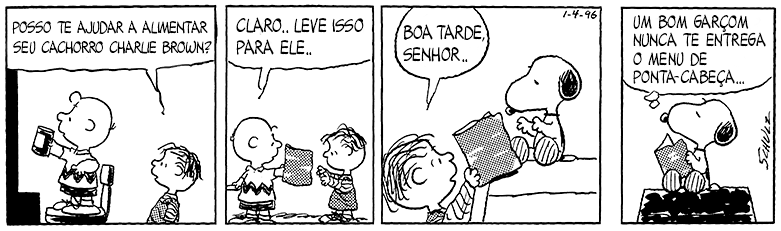
\includegraphics[scale=.5]{figuras/figura1}
        \fonte{Autoria própria.}
    \end{figure}

    Já na \cref{fig:figura2}, temos a mesma figura anterior, mas agora de forma quebrada em subfiguras, usando os ambientes \emph{figure} e \emph{subfigure}. Em \subref{fig:figura2a} temos a primeira parte, em \subref{fig:figura2b} temos a segunda parte, em \subref{fig:figura2c} temos a terceira parte, e em \subref{fig:figura2d} temos a quarta parte da figura. Caso deseje escrever algum rótulo ao lado das letras indicativa de uma subfigura, basta especificá-lo no comando \emph{caption} desta. Para omitir as letras (a), (b), (c) e (d), basta utilizar o comando \emph{caption*} em cada subfigura.

    \begin{figure}[!htb]
        \centering
        \caption{Exemplo de subfiguras}
        \label{fig:figura2}
    
        \begin{subfigure}{.29\textwidth} % Entre chaves, especificar a largura do espaço destinado à subfigura
            \centering
            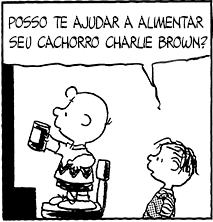
\includegraphics[scale=.5]{figuras/figura2a}
            \caption{}
            \label{fig:figura2a}
        \end{subfigure}
        %
        \begin{subfigure}{.19\textwidth}
            \centering
            
\includegraphics[scale=.5]{figuras/figura2b}
            \caption{}
            \label{fig:figura2b}
        \end{subfigure}
        %
        \begin{subfigure}{.29\textwidth}
            \centering
            
\includegraphics[scale=.5]{figuras/figura2c}
            \caption{}
            \label{fig:figura2c}
        \end{subfigure}
        %
        \begin{subfigure}{.19\textwidth}
            \centering
            
\includegraphics[scale=.5]{figuras/figura2d}
            \caption{}
            \label{fig:figura2d}
        \end{subfigure}
    
        \fonte{Autoria própria.}
    \end{figure}

    A fonte das figuras (e isso também vale para demais elementos como gráficos, tabelas, quadros etc.) deve estar especificada corretamente. Neste modelo, como trata-se apenas de exemplos, todas as fontes estão como ``Autoria própria''.